\chapter{Arrival Time Prediction}
\label{cha:arrival-time-prediction}

Trajectory forecasting is the process of predetermining when a bus arrives at a particular bus stop.
The existing arrival time prediction of Östgötatrafiken AB is based purely on long-time historical data.
It provides a single timestamp when it predicts the bus to arrive at a certain bus stop.
The prediction is the most likely arrival time for the bus.

This chapter uses a methodology similar to the previous Chapter \ref{cha:GPS-variation-estimation}.
The aim is to provide a probability distribution of arrival times for the next bus stops.
This thesis project proposes a Trajectory Forecasting model based on multiple GPs.
It provides time-to-arrival probability distributions for all the remaining bus stops in the journey.
The probability distribution allows for queries such as:
\begin{itemize}
    \item \textit{What is the most likely time of arrival at bus stop $p$ from the previous bus stop?}
    \item \textit{What is the probability of the bus arriving at the earliest/latest possible time?}
\end{itemize}

\section{Initial Methodology} \label{sec:initial-methodology}
The first steps of the proposed approach is similar to the steps covered in the Sections \ref{sec:stop-compression}-\ref{sec:segment-self-overlapping-journeys}.
Below is a brief description of the steps already covered, with alterations highlighted:

\begin{enumerate}
    \item \textit{Stop Model and Compression:}
    Stops during the trajectory are modelled as bus stops and red lights, i.e., common stops during a bus journey.
    GPS positions of stopped buses need to be compressed in order to support more robust GPs \cite{Tiger2018-gp-motion-pattern}.
    The result of this step is a collection of trajectories for each bus line.
    The trajectories include common stops and compressed GPS positions during stops.
    As in Section \ref{sec:stop-compression}, a \textit{Speed} threshold value of $0.1$ m/s is used for the trajectory forecasting.
    However, while stops due to traffic and red lights are compressed by removing positions occurring during a stop, they are not compressed time-wise.
    This means that the position before the stop and after the stop have potentially wildly different timestamps.
    The reason behind this is to indirectly model traffic and red lights as latent variables.
    The effects of traffic and red lights are neither explicitly modelled nor discarded.

    \item \textit{Synchronising Input Space:}
    The input space is synchronised using by training a global GP model $f_1$, given by eq. \ref{eq:gps-var-f1} in Section \ref{sec:synchronisation}.
    The model is thus
    \begin{equation} \label{eq:gps-var-f1}
        f_1: (x, y) \longmapsto \tau,
    \end{equation}
    and is implemented using the GPflow \cite{GPflow2017} framework.
    The training trajectory is distance filtered with a threshold of $6 \times 10^{-5}$, which roughly corresponds to a few metres.
    The GP is implemented using a RBF kernel with Automatic Relevance Determination (ARD) for the length-scale parameter.
    The data noise variance parameter $\sigma^2_n$ is fixed at $10^{-5}$.
    The $f_1$ GP is thus the same as the one used in Chapter \ref{cha:GPS-variation-estimation}.

    \item \textit{Segment Self-Overlapping Journeys:}
    Self-overlapping trajectories are segmented until no self-overlapping is occurring for the trajectory.
    The segmentation is required in order to avoid problems with instability, as mention in Section \ref{sec:self-overlapping-trajectories}, and the problem of overlapped positions in a model being trained to predict completely different arrival times.

    Each segment can potentially have a small model overlap, which means that neighbouring segments share a few data points.
    This improves the robustness of the model, as it retains the desired shape close to the borders \cite{Tiger2018-gp-motion-pattern}.
    The overlap used in this thesis project is set to five \texttt{ObservedPositionEvent}s, which is roughly 6.5\% of an average-length segment (around 77 \texttt{ObservedPositionEvent}s).

    \item \textit{Remove First Segment:}
    As briefly discussed in Chapter \ref{cha:GPS-variation-estimation}, the performance of the $f_1$ GP is poor when training on the start of the trajectory.
    Therefore, the first segment is removed from all trajectories.

\end{enumerate}

Once these three steps are executed, the approach diverges compared to the approach described in Chapter \ref{cha:GPS-variation-estimation}.

\section{Segment Bus Stops}
The trajectory is segmented at bus stops, which means that the \texttt{ObservedPositionEvent}s occurring between two bus stops are segmented into one \textit{trajectory segment}.
For example, a bus line $A\rightarrow B\rightarrow C$ is segmented into two segments
\begin{enumerate}
    \item $A\rightarrow B$
    \item $B\rightarrow C$
\end{enumerate}
The positions occurring during a bus stops are already compressed by Step 1 in Section \ref{sec:initial-methodology}.
While creating the segments, the arrival time for each segment is extracted from the trajectory.
The arrival time is the timestamp of the event where the system determines that the bus has reached the bus stop, e.g., the date when the bus reaches 
\begin{enumerate}
    \item $B$, after departing from bus stop $A$
    \item $C$, after departing from bus stop $B$
\end{enumerate}

Figure \ref{fig:segments} shows an example of the bus stop segmentation for an arbitrary trajectory.
Four sequential segments are visualised, with the relative time (in seconds) for each segment on the X-axis and the speed (m/s) of \texttt{ObservedPositionEvent}s on the Y-axis.

\begin{figure}
    \centering
    \begin{subfigure}[b]{0.475\textwidth}
        \centering
        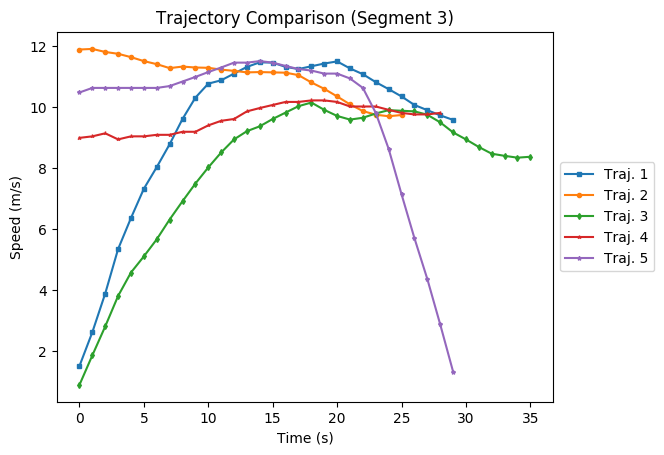
\includegraphics[width=\textwidth]{figures/speed_comparison_3}
        \caption[Segment1]%
        {{\small Segment 3}}    
        \label{fig:segment-1}
    \end{subfigure}
    \hfill
    \begin{subfigure}[b]{0.475\textwidth}  
        \centering 
        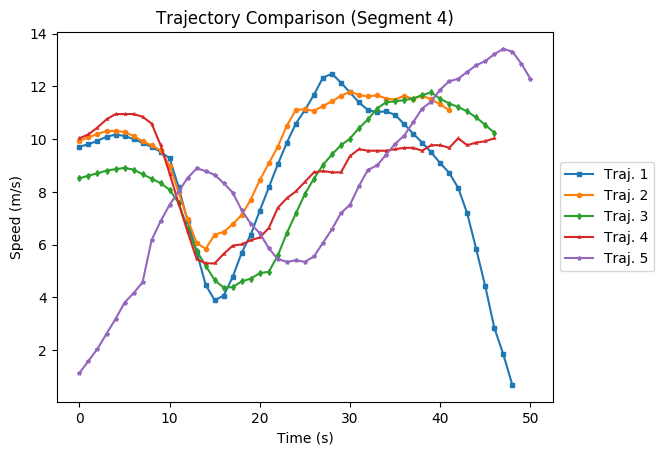
\includegraphics[width=\textwidth]{figures/speed_comparison_4}
        \caption[]%
        {{\small Segment 4}}    
        \label{fig:segment-2}
    \end{subfigure}
    \vskip\baselineskip
    \begin{subfigure}[b]{0.475\textwidth}   
        \centering 
        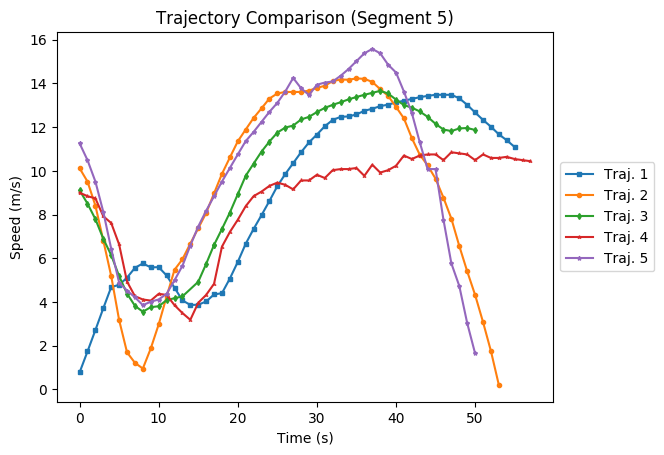
\includegraphics[width=\textwidth]{figures/speed_comparison_5}
        \caption[]%
        {{\small Segment 5}}    
        \label{fig:segment-3}
    \end{subfigure}
    \quad
    \begin{subfigure}[b]{0.475\textwidth}   
        \centering 
        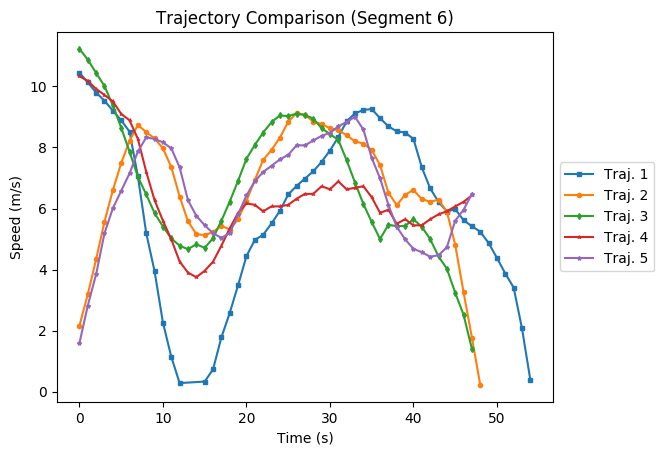
\includegraphics[width=\textwidth]{figures/speed_comparison_6}
        \caption[]%
        {{\small Segment 6}}    
        \label{fig:segment-4}
    \end{subfigure}
    \caption[ Example of trajectory segments ]
    {{\small Example of four trajectory segments with zero segment overlap.
    The X-axis is the relative time (in seconds) of the trajectory segment, the Y-axis is the speed of each \texttt{ObservedPositionEvent} point.
    Five trajectories are visualised for each segment.}} 
    \label{fig:segments}
\end{figure}

The result of the bus stop segmentation step is a collection of segments and segment arrival times for each trajectory.

\section{Trajectory Segment Forecasting Models}
The collection of segments and arrival times are used to create features for the arrival time prediction model.
Two different GP models are created and are given by
\begin{align}
    f_A&: \tau \mapsto t_s \label{eq:f_A} \\
    f_B&: (\tau, v) \mapsto t_s \label{eq:f_B}
\end{align}
\begin{itemize}
    \item $\tau$ is the trajectory progress for the bus. $\tau$ is calculated by using GP $f_1$ from eq. \ref{eq:gps-var-f1}.
    \item $t_s$ is the predicted arrival time to the bus stop at the end of segment $s$.
    \item $v$ is the speed of the bus at $\tau$. 
\end{itemize}  

\subsection{Model Comparison $f_A$ and $f_B$}
\begin{figure}[t]  
    \centering 
    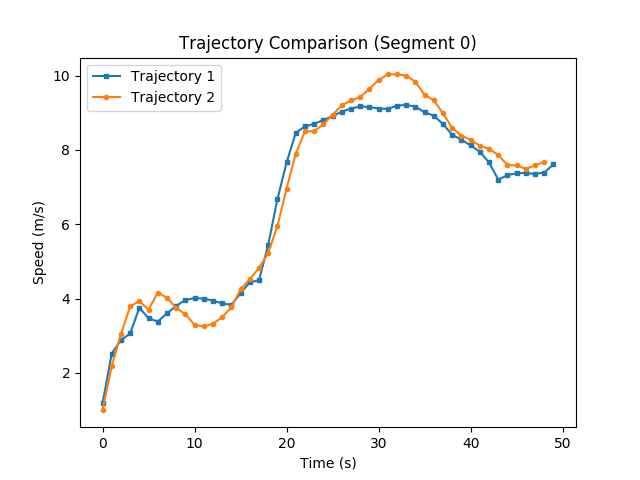
\includegraphics[width=\textwidth]{figures/speed_fB_comparison}
    \caption[ Trajectory comparison for segment $S_0$ ]%
    {{\small Trajectory comparison for segment $S_0$.
    Trajectory 1 is used to train $f^{(1)}_{B_0}$.
    Trajectory 2 is used to train $f^{(2)}_{B_0}$.
    Trajectory 1 is also used to evaluate both $f^{(1)}_{B_0}$ and $f^{(2)}_{B_0}$.}}   
    \label{fig:trajectory-comparison-s0}
\end{figure}

\begin{table}
    \centering
    \caption[Arrival time prediction with the $f_B$ GP model]%
    {{\small Arrival time prediction with the $f_B$ GP model.
    The GP model predicts the arrival time for a bus driving in segment $S_0$.
    This table contains only a part of segment $S_0$ .
    Two GP models trained on segment $S_0$ are used for the prediction: $f^{(1)}_{B_0}$ and $f^{(2)}_{B_0}$.
    The right column contains the true arrival time (in seconds remaining) for the bus.}}
    \label{table:f_B-examples} 
    \begin{tabular}{ |l|l|c| } 
        \hline
        Prediction $f^{(1)}_{B_0}(S_0)$ & Prediction $f^{(2)}_{B_0}(S_0)$ & Truth $S_0$ \\ [0.5ex] 
        \hline
        48.00032032 & -176.47767445 & 48.0 \\
        46.99899913 & -207.23221327 & 47.0 \\
        46.00140604 & -233.29939699 & 46.0 \\
        44.99743229 & -263.30660917 & 45.0 \\
        44.00544805 & -291.29058078 & 44.0 \\
        42.97906806 & -326.62038041 & 43.0 \\
        42.0257244 & -339.44856005 & 42.0 \\
        40.97131472 & -358.31354569 & 41.0 \\
        40.15149734 & -374.08468248 & 40.0 \\
        39.18597533 & -377.21521534 & 39.0 \\
        38.1260134 & -385.63015598 & 38.0 \\
        36.86945791 & -383.52959391 & 37.0 \\
        35.6697429 & -378.47844965 & 36.0 \\
        35.02909338 & -382.12072838 & 35.0 \\
        33.72776512 & -408.53070845 & 34.0 \\
        33.26752095 & -410.33279089 & 33.0 \\
        31.99396506 & -441.67817682 & 32.0 \\ 
        \hline
    \end{tabular}
\end{table}

\begin{table}
    \centering
    \caption[Arrival time prediction with the $f_A$ GP model]%
    {{\small Arrival time prediction with the $f_A$ GP model.
    The GP model predicts the arrival time for a bus driving in segment $S_0$.
    This table contains only a part of segment $S_0$.
    Two GP models trained on segment $S_0$ are used for the prediction: $f^{(1)}_{A_0}$ and $f^{(2)}_{A_0}$.
    The right column contains the true arrival time (in seconds remaining) for the bus.}}
    \label{table:f_A-examples} 
    \begin{tabular}{ |l|l|c| } 
        \hline
        Prediction $f^{(1)}_{A_0}(S_0)$ & Prediction $f^{(2)}_{A_0}(S_0)$ & Truth $S_0$ \\ [0.5ex] 
        \hline
        27.95503975 & 65.03012452 & 48.0 \\
        27.37264309 & 65.60988244 & 47.0 \\
        26.79024643 & 66.27802379 & 46.0 \\
        26.20784977 & 66.57825337 & 45.0 \\
        25.6254531 & 66.56967009 & 44.0 \\
        25.04305644 & 66.45871024 & 43.0 \\
        24.46065978 & 66.43164454 & 42.0 \\
        23.87826312 & 66.55277654 & 41.0 \\
        23.29586646 & 66.51186703 & 40.0 \\
        22.7134698 & 64.80122062 & 39.0 \\
        22.13107314 & 60.54143875 & 38.0 \\
        21.54867647 & 56.10481638 & 37.0 \\
        20.96627981 & 52.76073634 & 36.0 \\
        20.38388315 & 50.551963 & 35.0 \\
        19.80148649 & 49.37658565 & 34.0 \\
        19.21908983 & 48.68000806 & 33.0 \\
        18.63669317 & 47.65352869 & 32.0 \\
        \hline
    \end{tabular}
\end{table}

A comparison between GP models $f_A$ and $f_B$ is executed in order to find the best model for arrival time prediction.
In the comparison, both GP models use a Matérn kernel with $\nu =3/2$.

Table \ref{table:f_B-examples} shows the evaluation results of GP model $f_B$.
GP model $f_B$ is used to predict the arrival time for a particular bus driving in segment $S_0$.
GP model $f^{(1)}_{B_0}$ is trained with the same trajectory as both GP models are evaluated with.
GP model $f^{(2)}_{B_0}$ is trained on a different trajectory.
A comparison between the two trajectories used for the training of $f^{(1)}_{B_0}$ and $f^{(2)}_{B_0}$, respectively, is shown in Figure \ref{fig:trajectory-comparison-s0}.
Trajectory 1 is used for the training of GP model $f^{(1)}_{B_0}$, while trajectory 2 is used for the training of $f^{(2)}_{B_0}$.
Trajectory 1 is used for the evaluation of both models.
The results from the GP model $f^{(0)}_{B_0}$ does not come with any surprises, as the model is trained on the same data used to evaluate it.
However, GP model $f^{(2)}_{B_0}$ performs extremely poorly on unseen data; which is an indication that the model does not generalise well.
On the other hand, the two trajectories do not differ by much, as shown in Figure \ref{fig:trajectory-comparison-s0}.
This suggests that the model, kernel and/or kernel parameters are chosen poorly for the features used in $f_B$.

Table \ref{table:f_A-examples} show the evaluation results of GP model $f_A$.
The same approach is used in the evaluation:
\begin{itemize}
    \item Both models are evaluated on the same data
    \item GP model $f^{(1)}_{A_0}$ is trained on the same data used for the evaluation.
    \item GP model $f^{(2)}_{A_0}$ is trained on different data, but for the same segment $S_0$.
    \item The right column contains the true arrival times for the evaluation data.
\end{itemize}

It is surprising that the $f^{(1)}_{A_0}$ performs poorly when evaluated on training data.
However, as both models perform moderately well on both testing and training data, the $f_A$ model is the focus for the remainder of this thesis project.
Different kernels are tested and evaluated for the $f_A$, together with varying the hyperparameters.
The follow kernels are tested:

\newpage
\begin{enumerate}
    \item Linear
    \item White
    \item RBF
    \item RBF+Linear
    \item Matern32
\end{enumerate}
The different $f_A$ models are compared by calculating the following two metrics for each model:
\begin{enumerate}
    \item Root Mean Square Error (RMSE)
    \item Mean Absolute Error (MAE)
\end{enumerate}
The evaluation is similar to the evaluation between GP models $f_B$ and $f_A$.

The metric scores and the visual representation of the different GPs are taken into consider when choosing the best, appropriate model.
The best setting is used for the remainder of the thesis project.
GPflow also supports a wide range of optimisation algorithms.
This thesis project uses the standard L-BFGS-B algorithm.

\subsection{Model Evaluation $f_A$}
The results of the $f_A$ GP model evaluation are presented in Table \ref{table:metric-scores}.
The RBF kernel and the combined RBF+Linear kernel achieved the best scores.
While GPflow optimises the hyperparameters of the model, the optimisation occasionally gets stuck in a local minima.
The choice of initial kernel parameters is important, as a poor local minima in the optimisation function can result in poor robustness of a GP model.
While the kernels work equally well in the general case, there are segments where neither work, depending on the trajectory and initialisation, which is expected.
The problem with poor performance can be solved by, for example, changing the hyperparameter initialisation or varying it by using random restarts.
Figure \ref{fig:10-22-models} shows a comparison between the two kernels for two different segments, both with optimised initial parameters, which results in a better model comparison.
Both kernels produce similar models in the optimal case, with few differences.
Figure \ref{fig:10-7-rbf-linear} seems slightly better than the RBF kernel counterpart in Figure \ref{fig:10-7-rbf}, as the RBF+Linear kernel captures the linearity better in the start of the segment.
Manual analysis of the different segments show that most segments follow a linear trend with occasional curvature.
This suggests that a RBF+Linear kernel can be more suitable in the general case. 

\begin{table}
    \centering
    \caption[Metric scores for $f_A$ GP models]%
    {{\small Metric scores for $f_A$ GP models.
    The GP models predict the arrival time for a bus driving in segment $S_0$.
    The metrics are calculated by comparing the predicted arrival time to the true arrival time. 
    Two GP models are trained for each choice of kernel. 
    The model $f^{(1)}_{A_0}$ is trained on the same data as it is evaluated by.
    Model $f^{(2)}_{A_0}$ is evaluated on the same data as $f^{(1)}_{A_0}$, but is trained on different data.}}
    \label{table:metric-scores} 
    \begin{tabular}{ |c|r|r|r|r| } 
        \hline
        Kernel & RMSE $f^{(1)}_{A_0}$ & RMSE $f^{(2)}_{A_0}$ & MAE $f^{(1)}_{A_0}$ & MAE $f^{(2)}_{A_0}$ \\ [0.5ex] 
        \hline
        Linear & 24.85 & 25.26 & 20.56 & 21.49 \\
        White & 26.80 & 26.80 & 22.38 & 22.38 \\
        RBF & \textbf{1.56} & \textbf{13.53} & \textbf{0.84} & \textbf{11.69} \\
        RBF+Linear & \textbf{1.56} & 13.60 & \textbf{0.84} & 11.84 \\
        Matern32 & 11.19 & 13.56 & 9.34 & 11.75 \\
        \hline
    \end{tabular}
\end{table}

\begin{figure}
    \centering
    \begin{subfigure}[b]{0.475\textwidth}
        \centering
        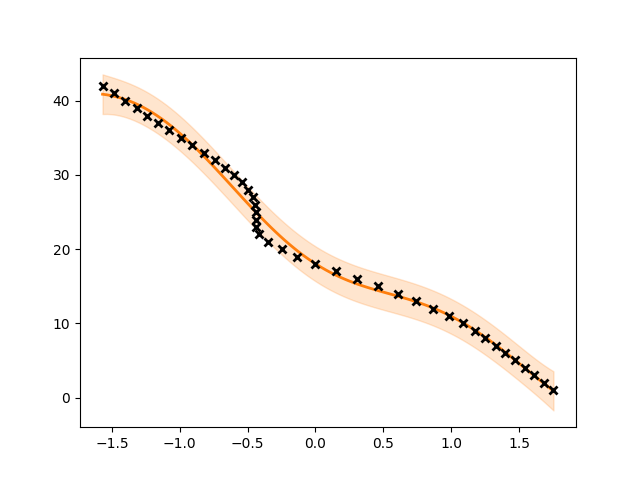
\includegraphics[width=\textwidth]{figures/forecasting/10_7_rbf}
        \caption[]%
        {{\small Model of trajectory 10, segment 7, using the RBF kernel.}}    
        \label{fig:10-7-rbf}
    \end{subfigure}
    \hfill
    \begin{subfigure}[b]{0.475\textwidth}  
        \centering 
        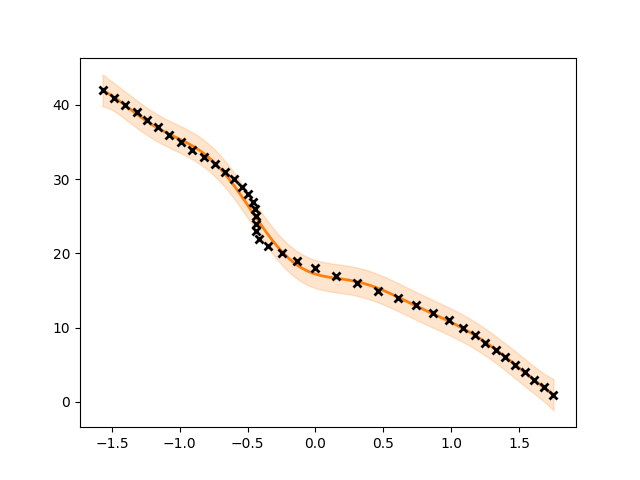
\includegraphics[width=\textwidth]{figures/forecasting/10_7_rbf_linear}
            \caption[]%
            {{\small Model of trajectory 10, segment 7, using the RBF+Linear kernel.}}    
            \label{fig:10-7-rbf-linear}
        \end{subfigure}
        \vskip\baselineskip
        \begin{subfigure}[b]{0.475\textwidth}   
            \centering
            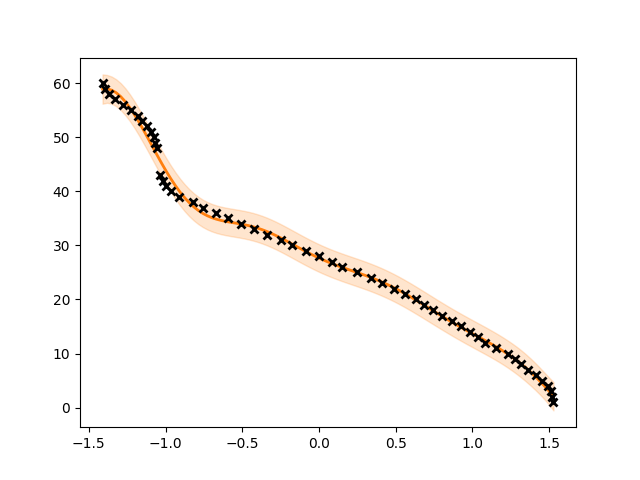
\includegraphics[width=\textwidth]{figures/forecasting/22_12_rbf}
            \caption[]%
            {{\small Model of trajectory 22, segment 12, using the RBF kernel.}}    
            \label{fig:22-12-rbf}
        \end{subfigure}
        \quad
        \begin{subfigure}[b]{0.475\textwidth}   
            \centering 
            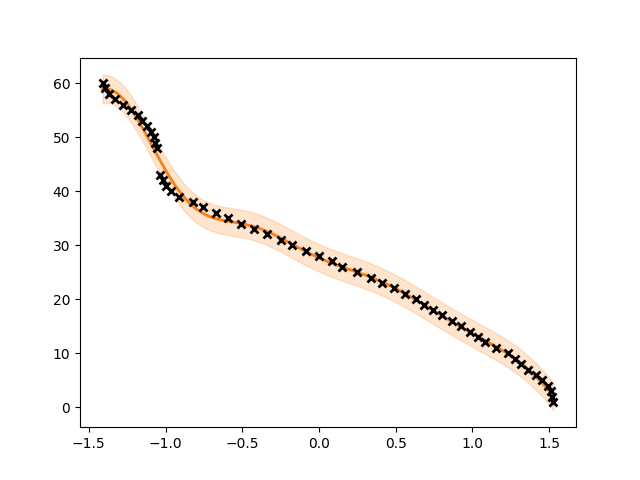
\includegraphics[width=\textwidth]{figures/forecasting/22_12_rbf_linear}
            \caption[]%
            {{\small Model of trajectory 22, segment 12, using the RBF+Linear kernel.}}    
            \label{fig:22-12-rbf-linear}
        \end{subfigure}
        \caption[ Visualisation of $f_A$ models with different kernels ]
        {{\small Visualisation of $f_A$ models with different kernels.
        Each figure contains the predictive mean and variance of the model, alongside the training data points.  
        The X-axis is the $\tau$ values of the trajectory segment and the Y-axis is the arrival time to the end of the segment, in seconds.}} 
        \label{fig:10-22-models}
    \end{figure}

% \begin{figure}
%     \centering
%     \begin{subfigure}[b]{0.475\textwidth}   
%         \centering
%         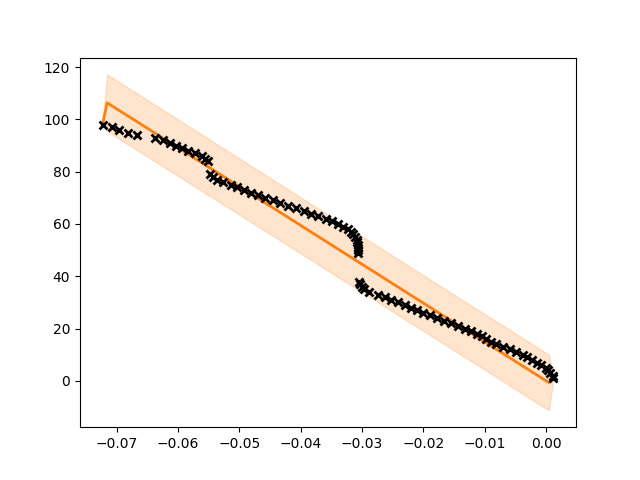
\includegraphics[width=\textwidth]{figures/forecasting/gp_3_18_rbf_linear_log}
%         \caption[RBF+Linear kernel with logarithmised input.]%
%         {{\small RBF+Linear kernel with logarithmised input. 
%         The model is trained on data from trajectory 3, segment 18.
%         }}
%         \label{fig:3-18-log}
%     \end{subfigure}
%     \quad
%     \begin{subfigure}[b]{0.475\textwidth}   
%         \centering 
%         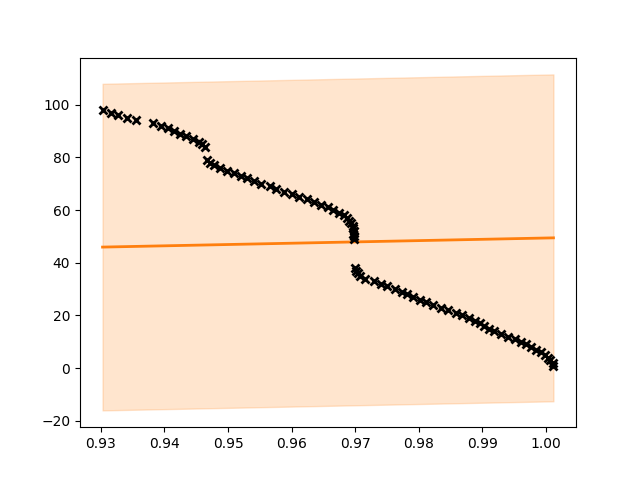
\includegraphics[width=\textwidth]{figures/forecasting/gp_3_18_linear}
%         \caption[Linear kernel component of the RBF+Linear model.]%
%         {{\small Linear kernel component of the RBF+Linear model. 
%         The model is trained on data from trajectory 3, segment 18.
%         }}
%         \label{fig:3-18-linear}
%     \end{subfigure}
%     \caption[ Visualisation of arbitrary segments with the RBF+Linear kernel ]
%     {{\small Visualisation of segments with the RBF+Linear kernel.
%     Each figure contains the predictive mean and variance of the model, alongside the training data points.  
%     The X-axis is the $\tau$ values of the trajectory segment and the Y-axis is the arrival time to the end of the segment, in seconds.}} 
%     \label{fig:3-18-variations}
% \end{figure}

% Figure \ref{fig:3-18-log} shows how the model in \ref{fig:3-18-rbf-linear} performs better if the natural logarithm is applied to the input data.
% The improved performance indicates that the RBF+Linear model performs better if the input values are closer, or around zero.
% In Figure \ref{fig:3-18-linear}, only the Linear kernel component from the RBF+Linear model shown in Figure \ref{fig:3-18-rbf-linear} is visualised.
% The figure indicates that the Linear kernel component takes over the combined kernel.
% In order to try and resolve the problems, the initial hyperparameters of the RBF+Linear model are varied manually, until a stable model is acquired.
\newpage
\subsection{Final Model}
Figure \ref{fig:good-kernel-results} shows the final RBF+Linear model with the following initial hyperparameters:
\begin{enumerate}
    \item $l_{RBF}=0.1$, where $l_{RBF}$ is the length-scale of the RBF kernel in the combined RBF+Linear model.
    \item $\sigma_{Linear}^2=500$, where $\sigma_{Linear}^2$ is a prior on the variance of the Linear kernel in the combined RBF+Linear model.
\end{enumerate}

\begin{figure}
    \centering
    \begin{subfigure}[b]{0.475\textwidth}   
        \centering
        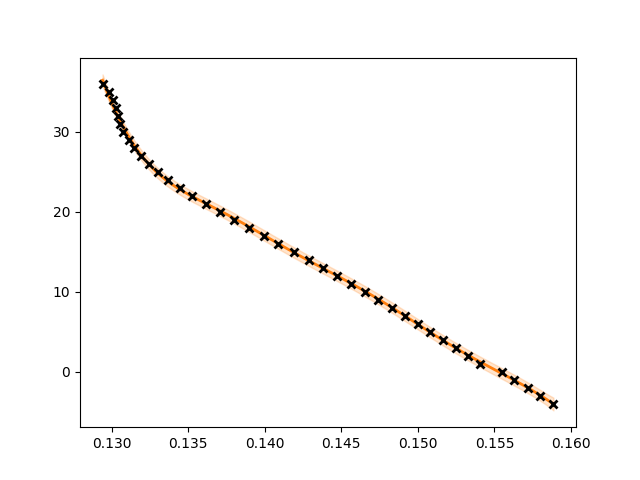
\includegraphics[width=\textwidth]{figures/forecasting/gp_16_4_rbf_linear}
        \caption[]%
        {{\small Model of trajectory 16, segment 4, using the RBF+Linear kernel.}}    
        \label{fig:16-4-rbf-linear}
    \end{subfigure}
    \quad
    \begin{subfigure}[b]{0.475\textwidth}   
        \centering 
        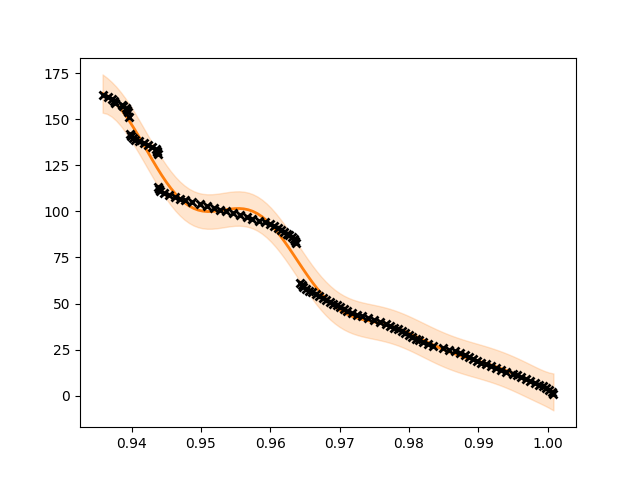
\includegraphics[width=\textwidth]{figures/forecasting/gp_26_18_rbf_linear}
        \caption[]%
        {{\small Model of trajectory 26, segment 18, using the RBF+Linear kernel.}}    
        \label{fig:26-18-rbf-linear}
    \end{subfigure}
    \caption[ Visualisation of arbitrary segments with the RBF+Linear kernel ]
    {{\small Visualisation of segments with the RBF+Linear kernel.
    Each figure contains the predictive mean and variance of the model, alongside the training data points.  
    The X-axis is the $\tau$ values of the trajectory segment and the Y-axis is the arrival time to the end of the segment, in seconds.}} 
    \label{fig:good-kernel-results}
\end{figure}

The arrival time prediction model is evaluated with the Leave-One-Out (LOO) approach:
\begin{enumerate}
    \item One trajectory from the pool of 38 trajectories used in the thesis is randomly chosen as a test trajectory.
    \item The test trajectory is used for evaluation on all $K-1$ models trained on different data.
    In this case, the test trajectory is used to evaluate 37 models.
    \item The first step is repeated, but with another trajectory.
\end{enumerate}

The evaluation is done by predicting the arrival time at each \texttt{ObservedPositionEvent} $p_i$ in the test trajectory.
Each model gives a predictive mean and variance for the arrival time.
The prediction is thus a mixture of Gaussian distributions.
The mixture is in this thesis project assumed to have a uniform prior.
The predicted arrival time is chosen to be the mean of the mixture means.

\begin{figure}
    \centering
    \begin{subfigure}[b]{0.475\textwidth}
        \centering
        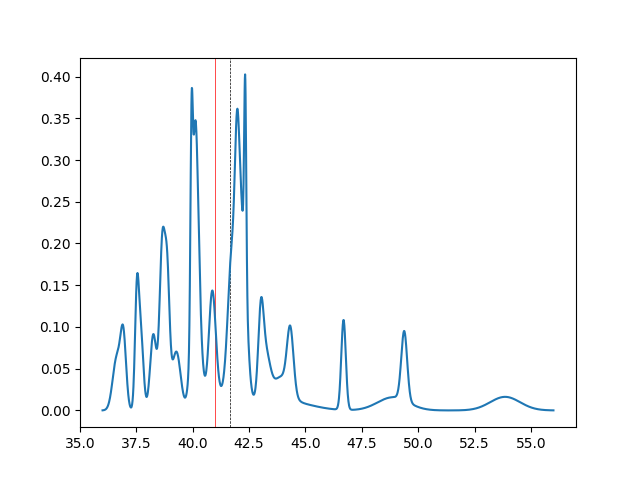
\includegraphics[width=\textwidth]{figures/arrival_times/res_5_traj32_seg4}
        \caption[]%
        {{\small Predicted arrival time for trajectory 32 at segment 4.
        The black dotted line is the mean predicted arrival time of the mixture.
        The red line is the true arrival time at that point in the segment.}}    
        \label{fig:result-1}
    \end{subfigure}
    \hfill
    \begin{subfigure}[b]{0.475\textwidth}  
        \centering 
        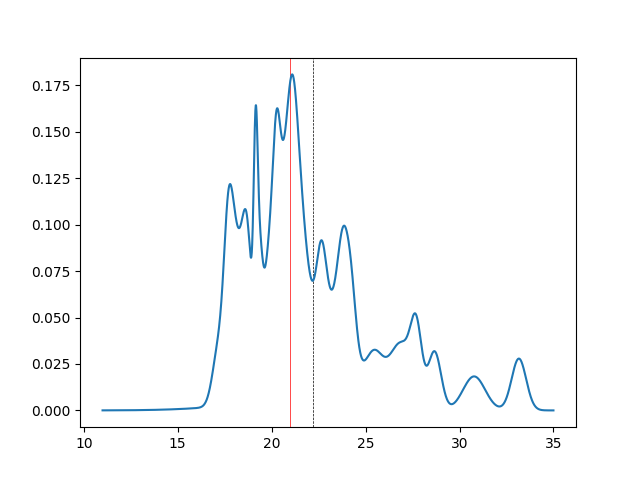
\includegraphics[width=\textwidth]{figures/arrival_times/res_10_traj13_seg10}
            \caption[]%
            {{\small Predicted arrival time for trajectory 13 at segment 10.
            The black dotted line is the mean predicted arrival time of the mixture.
        The red line is the true arrival time at that point in the segment.}}    
        \label{fig:result-2}
    \end{subfigure}
    \vskip\baselineskip
    \begin{subfigure}[b]{0.475\textwidth}   
        \centering
        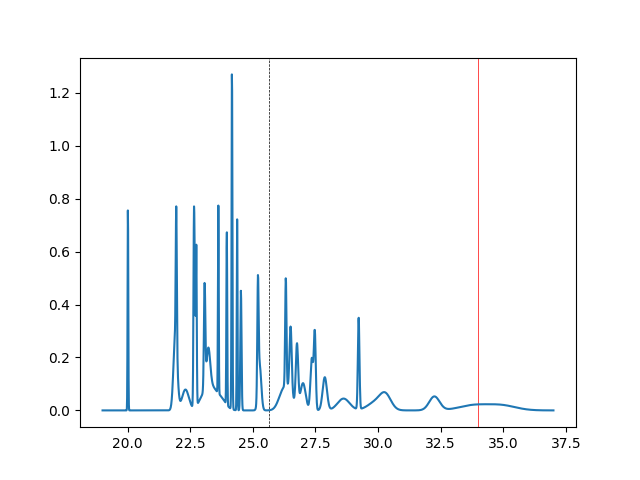
\includegraphics[width=\textwidth]{figures/arrival_times/res_5_traj17_seg3}
        \caption[]%
        {{\small Predicted arrival time for trajectory 17 at segment 3.
        The black dotted line is the mean predicted arrival time of the mixture.
        The red line is the true arrival time at that point in the segment.}}    
        \label{fig:result-3}
    \end{subfigure}
    \quad
    \begin{subfigure}[b]{0.475\textwidth}   
        \centering 
        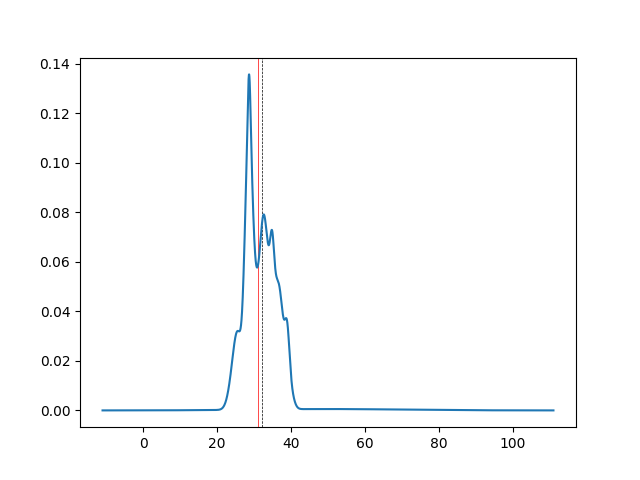
\includegraphics[width=\textwidth]{figures/arrival_times/res_12_traj13_seg7}
        \caption[]%
        {{\small Predicted arrival time for trajectory 13 at segment 7.
        The black dotted line is the mean predicted arrival time of the mixture.
        The red line is the true arrival time at that point in the segment.}}    
        \label{fig:result-4}
    \end{subfigure}
    \caption[ Predicted arrival times ]
    {{\small Predicted arrival times.
    Each figure contains the predictive and true arrival time for the test trajectory, evaluating on 37 models trained on different trajectories.
    The dashed line is the predicted arrival time from the mixture of Gaussian distributions.
    The red line is the true arrival time.
    The X-axis is the arrival time to the end of the segment, in seconds.
    The Y-axis is the PDF of the Gaussian mixture. }} 
    \label{fig:arrival-times}
\end{figure}

The evaluation metrics for the model are presented in Table \ref{tab:arrival-time-eval-metrics}.
The RMSE and MAE is calculated for each bus stop segment and the table presents the mean and standard error of the metrics for all segments in a trajectory.
The score is calculated by taking the mean and standard error RMSE and MAE from all segments.
The standard error is given by 
\begin{equation}
    SE = \frac{\sigma}{\sqrt{n}},
\end{equation}
where $\sigma$ is the standard deviation calculated using Bessel's correction
\begin{equation}
    \sigma = \sqrt{\frac{\sum_{i=1}^n (x_i - \bar{x})^2}{n - 1}}
\end{equation}

\section{Results}
The arrival times for an arbitrary \texttt{ObservedPositionEvent} are shown in Figure \ref{fig:arrival-times}.
The dashed line is the predicted arrival time, the red line is the true arrival time.
The X-axis is the arrival time to the next bus stop, in seconds.
The Y-axis is the PDF of the Gaussian mixture.

Table \ref{tab:arrival-time-eval-metrics} shows the evaluation done at a segment level.
A segment is the route between two bus stops.
Each segment only predicts the arrival time to the end of that segment.
The RMSE and MAE is calculated for each segment, for each respective trajectory.
In these results the bus line has 18 segments.
The RMSE and MAE scores presented in Table \ref{tab:arrival-time-eval-metrics} is thus the mean RMSE and mean MAE of all 18 segments for each respective trajectory.
The standard error is calculated using Bessel's correction.

Table \ref{tab:arrival-time-metrics} presents the RMSE and MAE scores on a trajectory level.
The prediction is still done at a bus stop segment level.
However, instead of calculating the mean RMSE and MAE for all segments, the RMSE and MAE is calculated for the whole trajectory.

Figure \ref{fig:arrival-time-metric-timeline} shows how the absolute errors of the predicted arrival times decrease over time for arbitrary segments.

\begin{table}[h!]
    \centering
    \caption[ Evaluation of arrival time prediction model ]%
    {{\small Evaluation of arrival time prediction model.
    The RMSE and MAE is calculated for each segment in each trajectory.
    A segment is the route between two bus stops.
    The average RMSE and MAE score is shown, together with the standard error using Bessel's correction.
    This is the average for all segments in a trajectory.}}
    \label{tab:arrival-time-eval-metrics} 
    \begin{tabular}{ |c|r|r| }
        \hline
        Test Trajectory \# & RMSE [s] & MAE [s] \\
        \hline
        13 & 6.14 $\pm$ 1.9 & 5.18 $\pm$ 1.56\\
        17 & 4.71 $\pm$ 0.64 & 4.18 $\pm$ 0.57 \\
        18 & 7.22 $\pm$ 2.03 & 6.55 $\pm$ 2.0 \\
        22 & 3.86 $\pm$ 0.88 & 3.35 $\pm$ 0.78 \\
        32 & 7.47 $\pm$ 2.09 & 6.54 $\pm$ 1.81 \\
        35 & 5.68 $\pm$ 1.17 & 4.83 $\pm$ 1.06 \\
        \hline
    \end{tabular}
\end{table}

\begin{table}[h!]
    \centering
    \caption[ Evaluation of arrival time prediction model ]%
    {{\small Evaluation of arrival time prediction model.
    The RMSE and MAE is calculated for each trajectory.
    The arrival time predictions are still for segments in the trajectory.
    However, instead of calculating the scores for each segment, the scores are predicted for all arrival time predictions done during the trajectory.}}
    \label{tab:arrival-time-metrics} 
    \begin{tabular}{ |c|r|r| }
        \hline
        Test Trajectory \# & RMSE [s] & MAE [s] \\
        \hline
        13 & 16.94 & 10.8 \\
        17 & 5.93 & 4.84 \\
        18 & 19.52 & 12.79 \\
        22 & 5.92 & 4.0 \\
        32 & 19.04 & 12.44 \\
        35 & 12.4 & 8.5 \\
        \hline
    \end{tabular}
\end{table}

\begin{figure}[!ht]
    \centering
    \begin{subfigure}[b]{0.475\textwidth}
        \centering
        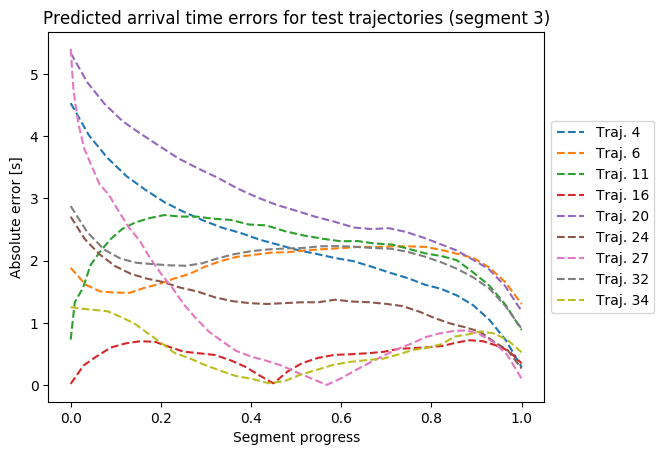
\includegraphics[width=\textwidth]{figures/metrics/segment_3}
        \caption[]%
        {{\small Absolute error for segment 3.}}    
        \label{fig:metric-result-1}
    \end{subfigure}
    \hfill
    \begin{subfigure}[b]{0.475\textwidth}  
        \centering 
        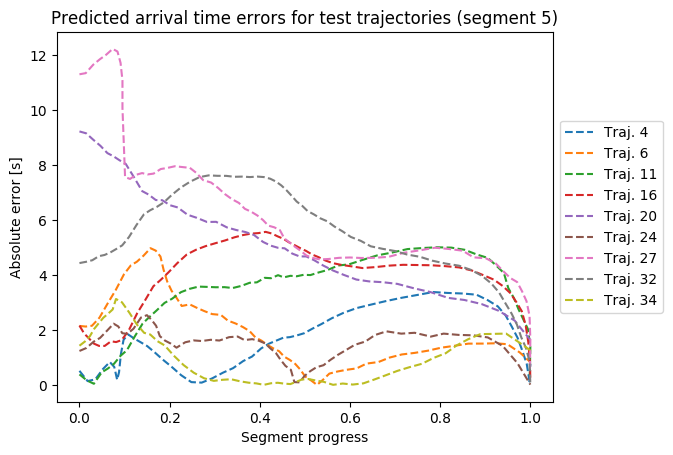
\includegraphics[width=\textwidth]{figures/metrics/segment_5}
            \caption[]%
            {{\small Absolute error for segment 5.}}    
        \label{fig:metric-result-2}
    \end{subfigure}
    \vskip\baselineskip
    \begin{subfigure}[b]{0.475\textwidth}   
        \centering
        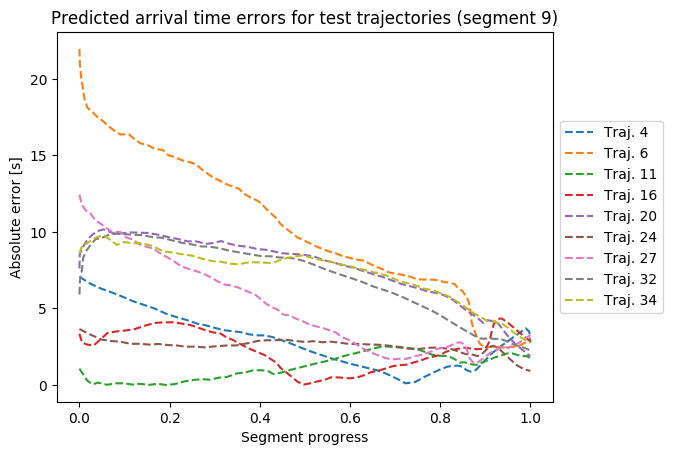
\includegraphics[width=\textwidth]{figures/metrics/segment_9}
        \caption[]%
        {{\small Absolute error for segment 9.}}    
        \label{fig:metric-result-3}
    \end{subfigure}
    \quad
    \begin{subfigure}[b]{0.475\textwidth}   
        \centering 
        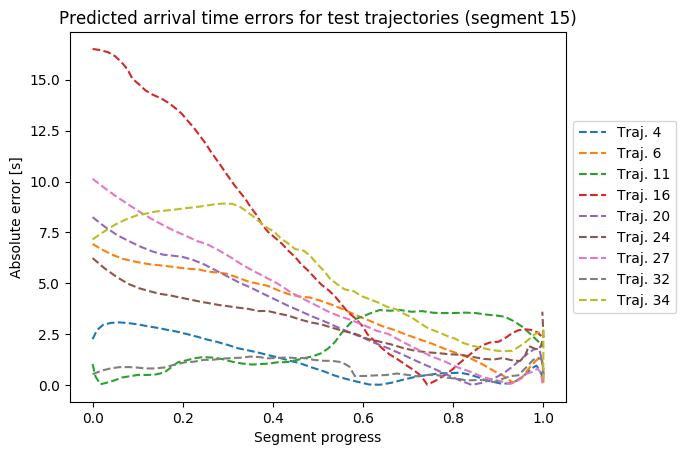
\includegraphics[width=\textwidth]{figures/metrics/segment_15}
        \caption[]%
        {{\small Absolute error for segment 15.}}    
        \label{fig:metric-result-4}
    \end{subfigure}
    \caption[ Absolute error of predicted arrival times for test trajectories. ]
    {{\small Absolute error of predicted arrival times for test trajectories.
    Each figure contains the absolute error of the predicted arrival time for each test trajectory in arbitrary segments.
    The X-axis is the segment progress from start of the segment to the end of the segment.
    The start and end of the segment are bus stops, as the segmentation is done on a bus stop level.}} 
    \label{fig:arrival-time-metric-timeline}
\end{figure}

\newpage
\section{Discussion}

The different evaluation methods highlight different aspects of the implemented model.
Table \ref{tab:arrival-time-eval-metrics} presents the RMSE and MAE scores at a segment level.
The segments are the route between two bus stops.
A trajectory is thus a collection of segments.
The scores presented in the table give an average measurement of the scores for all segments in a trajectory.
For certain test trajectories (17 and 22), all segments have a similar score, which causes the standard error to be lower.
Other test trajectories have segments with varying scores, resulting in higher standard error.
This is also reflected in Table \ref{tab:arrival-time-metrics}, which presents the RMSE and MAE scores at a trajectory level.
Individual segments are not used to calculate the scores.
The evaluation measures are thus an indication on how well, in general, the model predicts the arrival times for the tested trajectories.
The tested trajectories with higher RMSE and MAE scores in Table \ref{tab:arrival-time-metrics} also have higher standard errors in Table \ref{tab:arrival-time-eval-metrics}.

The use of RMSE and MAE to evaluate the performance of the arrival time prediction model does not cover all aspects of the model.
When calculating the overall RMSE and MAE scores for the whole trajectory, or for each segment respectively, they average errors occurring over time.
Figure \ref{fig:arrival-time-metric-timeline} shows how the absolute error decreases, in general, over time for each segment.
The model achieves better arrival time prediction as the buses travel the segment. 
The mean scores reflect poorly on the improvement over time, as the mean scores are heavily affected by the first few arrival time predictions done for each segment.
The poor scores in the beginning of each segment can be indicative of poor structure for the GP models.

The arrival time distribution created by the system has numerous benefits compared to a single, most probable, arrival time.
For example, the most likely arrival time can be calculated from the distribution either as a mixture mean, as in the naïve approach, or by using various methods \cite{Carreira2000, Comaniciu2002, Pulkkinen2013}
Furthermore, the probabilities of early arrival times and late arrival times can be calculated by integrating over the combined PDF from the model.

\subsection{Arrival Time Prediction Aggregation}
The aggregation of predicted arrival times used in this thesis project is too simple.
It is heavily affected by the number of models used and captures only the average of the predicted arrival times.
The assumption that the mixture of Gaussian distributions have a uniform prior is too naïve to give one correct prediction.
This is obvious in the results, as the quality of the prediction wildly vary depending on test trajectory.
The reason behind this is that while models do capture different trajectory behaviours for a single segment, e.g., heavy traffic compared with no traffic, the final prediction is only based upon the average of all models.
If the typical model is traffic-free, then the predicted time is skewed towards a traffic-free arrival time.
However, if a few trained models capture extreme traffic, then those predictions also affect the mean of all predicted arrival times.
The use of a mixture with an assumed uniform prior is thus too simple to result in good predictions.

A better approach is to calculate the \textit{data log likelihood} of a set of observed data points, given a GP model.
The data log likelihood can then be used as a weight for each model.
The larger the weight, the bigger the likelihood that the observed data is from a particular GP model.
In the example above, where the majority of models are traffic-free and a few model heavy traffic, a test trajectory with heavy traffic increases the weights of the predictions from the few models and reduces the weight of the predictions from the majority of the models.
The result is a better prediction of the arrival time.
This method can be used either on each observed data point, in order to see which model best describes that point, or on a trace of observer data points.
If a trace of observed data points are used instead, the weights would, over time, gravitate towards the models which best explain the observed data.
For example, in the predicted arrival time distribution shown in \ref{fig:result-3}, the naïve approach performs poorly compared to the other visualised results.
If the weighted approach is used instead, the idea would be that the modes closer to the red line would receive a larger weight than the majority of modes around the 20-27.5 second interval.

\subsection{Kernels}
Due to time limitations in the thesis project it is necessary to narrow down the model search space as development continued.
The choice of kernel is an important one.
The performance of the RBF kernel is similar to the RBF+Linear kernel. 
The hyperparameter initialisation might have caused the RBF+Linear kernel to perform slightly better.
The linear trend in the data can be removed by applying a de-trending method, e.g., differencing or model fitting.
This pre-processing step would have been beneficial for the RBF kernel, which might have caused better performance overall.

The hyperparameters of the kernels can also be optimised using HMC sampling, instead of the L-BFGS-B algorithm.
This could have avoided the local minima problems with the hyperparameters. 
It is a non-trivial problem to find a good initialisation for the hyperparameters, as they are used for over 700 GP models.
Any one of those GPs might get stuck in local minima, which would require changes to the hyperparameter initialisation.
The arrival time models took, on average, seven hours to train. 

In hindsight, the use of ARD should have been investigated for the $f_B$ model, where the \textit{Speed} is a part of the feature.
Using different kernels for different dimensions is also interesting to experiment with, as the model might capture new patterns.

\subsection{Common Stops}
Stop compression is the process of compressing common stops.
This can be done at different levels, depending on the definition of a common stop.
In this thesis project only bus stops are defined as common stops during the segmentation process, due to time limitations.
Only bus stops are considered as common stops since this is the simplest approach possible (beyond no segmentation at all).
The approach results in a probability distribution of arrival time predictions for the next bus stop.
With the improved arrival time aggregation, this approach also models red lights and traffic as latent variables.
The simplicity of the model is maintained, which makes the model easy to understand.
Unfortunately the complexity is increased in the arrival time aggregation.

Other possible definitions of common stops are:
\begin{enumerate}
    \item \textit{Bus Stops and Red Lights:}
    Modelling common stops using both bus stops and red lights would probably be the optimal approach.
    Red lights are static phenomenons which either causes a change to the expected arrival time (if red light) or not (green light).
    However, deciding whether or not a stop occurred due to red lights or traffic is not trivial with the data available in the dataset.
    Stops in all trajectories for the same bus line could be compared and a common ground could be established, but what would the comparison be?
    For example, if the same stop occurs in 90\% of all trajectories and it is not a bus stop, then it is most likely a red light, but how often does this occur?
    Maybe a more reasonable approach would be to combine the data with information from Google Maps Roads API or OpenStreetMap\footnote{https://www.openstreetmap.org/}, as they contain information about crossings with red lights.
    A crossing would then be more accurately labelled as having a red light or not, which could be used as input by the system.  
    Nevertheless, traffic would still be a latent variable not modelled by the extended approach.
    
    \item \textit{All Stops:}
    This extreme approach would model all stops in each trajectory as a common stop.
    The approach would create a larger number of segments compared to the previous, more restrictive, approaches.
    A trajectory suffering from heavy traffic would create multiple segments over a potentially short distance.
    The complexity of the model would thus explode as the number of segments grow.
    However, with a large dataset this approach could be effective to model the effects of traffic, but experiments are needed in order to determine the requirement on the dataset size. 
\end{enumerate}

\subsection{Red Lights}
If the second approach is applied to the arrival time prediction model, then valuable information could be gained by analysing the crossing with and without red lights.
Dedicated red lights exist for public transportation vehicles, which instantly turn green once a bus is arriving at the crossing.
By modelling crossings, the usefulness of such dedicated crossings could be investigated.
For example, crossings with abnormally long waiting times could be detected and dedicated traffic lights could be either tested or simulated for these crossings.
This information could prove to be a major benefit to the planning of roads and public transportation routes. 

\subsection{Poor Bus Stop Detection}
The poor bus stop detection algorithm resulted in bad arrival time prediction models when using the naïve arrival time aggregation method.
Figure \ref{fig:bad-gp-rese-c} illustrates a scenario where the position of the final bus has multiple modes, but the system does not register one of the modes as being part of the bus stop.
As a result, the bus stops at the bus stop for slightly over 3 minutes before driving past a mode which the system recognises.
As shown, this causes a large offset to occur in the arrival time prediction for the trained model.
The platform (mode) where the bus stops at is a dedicated waiting space and drop-off space for passengers.
As such, this platform should be included in the bus stop detection.
With an improved bus stop detection algorithm, such problems could have been avoided.

\begin{figure}[t]
    \centering
    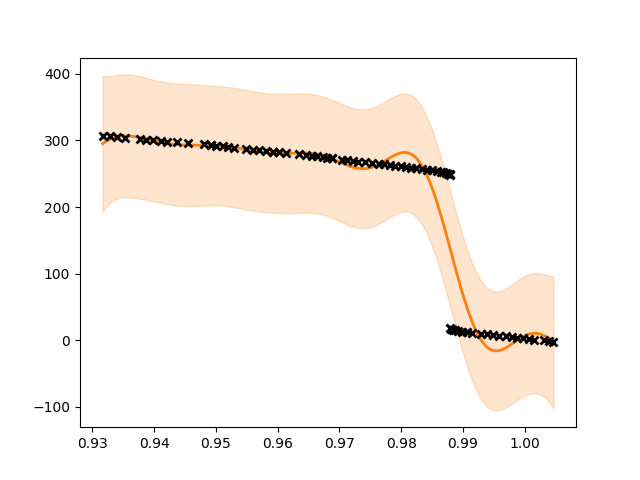
\includegraphics[width=0.9\textwidth]{figures/forecasting/bad_gp_rese_centrum}
    \caption[Example of poor bus stop detection for a bus stop with multiple modes]%
    {\small Example of poor bus stop detection for a bus stop with multiple modes.
    The Y-axis is the predicted arrival time.
    The X-axis is the segment progress.
    The black points are the true arrival times at each observed data point.
    The orange region is the predictive mean and variance of the trajectory forecasting model.
    The bus arrives to a platform dedicated to dropping off passengers.
    The bus stops at this platform for around 250 seconds.
    This platform is not registered as a part of the bus stop by the system, which causes a large offset in the predicted arrival times, as indicated by the red circle.
    The system registers the bus at the bus stop once the bus drives past the main mode (the main platform) of the bus stop.
    }
    \label{fig:bad-gp-rese-c}
\end{figure}

\subsection{Time and Day Model}
An interesting concept that should be explored is the addition of time and day to the model as a feature.
Different times of the day and different days are expected to exhibit different arrival time patterns.
For example, traffic is expected to be heavier in certain areas during rush hours and before holidays, while lighter on evenings and nights. 
Modelling this could improve the accuracy of the arrival time prediction models. 

\section{Future Work}
Future work on arrival time prediction (trajectory forecasting) should be focused on improving the arrival time prediction aggregation.
The weighted mixture method should be implemented and tested as a next step.
One could also experiment with the different approaches to model common stops, by adding information from external sources, as this could be beneficial information to have when planning routes and road improvements.
Naturally, more days from the dataset should be processed and added to the model, as this thesis project only utilised the data from one day.
The model should also be tested in comparison with the baseline available by Östgötatrafiken AB, by predicting the arrival time of buses in real-time, and compare with the prediction made by the existing system.

